% Chapter 1

\chapter{绪论}

\section{研究背景与意义}
近年来，无线通信与物联网技术的持续演进在一定程度上推动了社会信息化的进程，使得移动终端规模与数据流量呈现出稳步增长的趋势。根据中华人民共和国工业和信息化部发布的《2025年通信业统计公报》，截至2025年底，我国移动电话用户总数达到18.27亿户，全年移动互联网接入流量累计为3958亿GB，全国移动电话基站总数也已扩充至1287万个\upcite{miit2025}。
这些基础设施的建设与数据规模的增长，为虚拟现实\upcite{7946930}、增强现实\upcite{8329628}、自动驾驶\upcite{liu2021vehicular}等应用场景的落地提供了基本的网络环境。与此同时，此类新兴应用对计算能力和响应时延提出了更为具体的挑战。以自动驾驶辅助系统为例，其在运行过程中需要对周围环境数据进行及时的分析与处理，以协助完成安全决策。在远程医疗或工业协作场景中，网络延迟的波动往往会直接影响到任务的执行效率。然而，随着应用需求的日益多样化，在处理上述新兴业务时，传统的计算模式逐渐暴露出一些客观存在的局限性。首先，受限于便携式终端设备的物理尺寸与电池容量，其本地运算能力往往难以独立支撑复杂的计算任务。其次，
传统的云计算模式通过将计算任务传输至远端云服务器处进行处理并返回计算结果\upcite{8016573,patel2014mobile}。在应对高频率、低时延的任务处理时，这种计算模式将受限于长距离传输和中心化处理，暴露出资源分布不均或响应滞后等实际问题，难以满足某些对实时性要求较高的应用场景。

\begin{figure}[htbp]
	\centering
	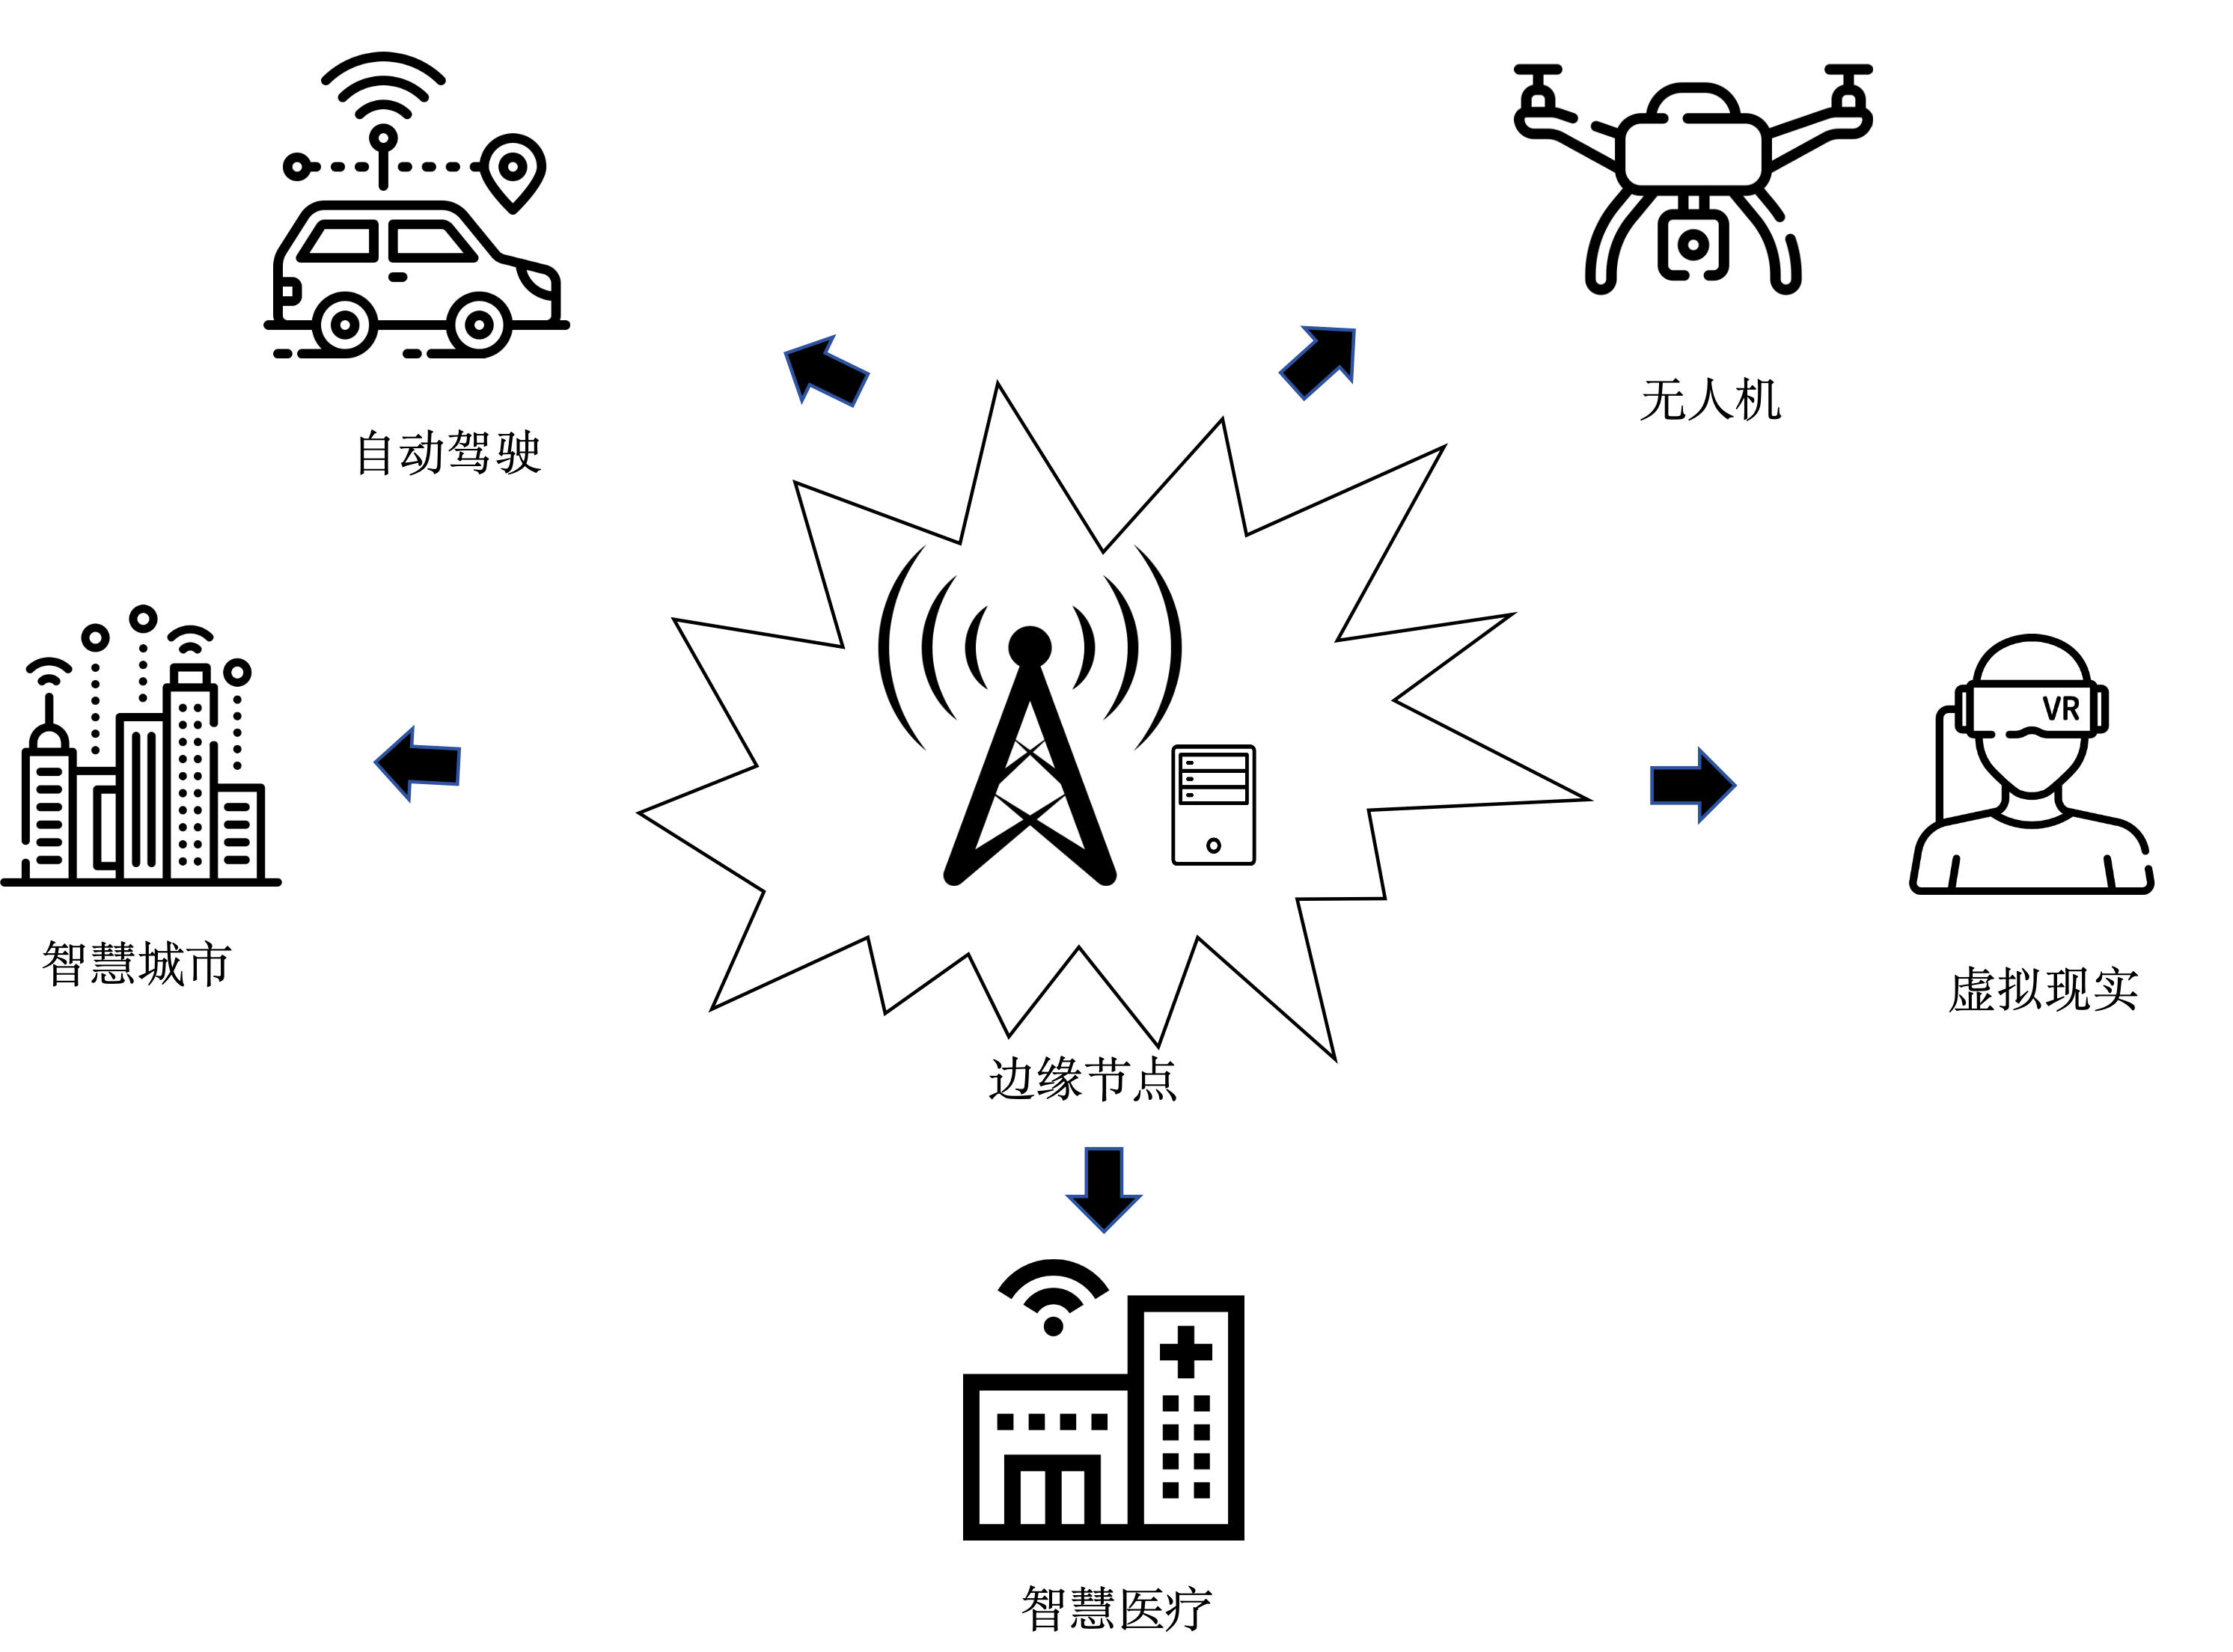
\includegraphics[width=0.6\textwidth]{figures/边缘计算示例图.png}
	\caption{边缘计算应用场景示意图}
	\label{fig-Edge-Computing-Application}
\end{figure}

针对这些实际需求，边缘计算作为一种新兴计算范式，受到了学术界与工业界的关注\upcite{8016573,patel2014mobile}。早在2014年，欧洲电信标准协会（European Telecommunications Standards Institute）正式提出了边缘计算的概念\upcite{patel2014mobile}。其核心思想是通过在网络边缘部署计算资源，使得移动设备可以将算力需求较高的任务卸载至网络边缘的节点上进行计算并回传计算结果，从而起到降低响应时延、缓解终端能耗压力的作用。目前，边缘计算已成为5G及未来移动通信网络中的关键技术方向之一，并在虚拟/增强现实\upcite{9363323,9789210}、自动驾驶\upcite{10213996,8584062}、无人机\upcite{9778241,uavassited}、智慧城市\upcite{10551400,9063670}、智慧医疗\upcite{10339657,11008531}等诸多领域获得了广泛应用。

然而，随着应用数据的持续激增以及计算任务的规模持续扩大（如智能驾驶\upcite{autodriving}，人工智能\upcite{10333824,10835069}等），单一节点的计算资源难以进一步支持大规模的计算任务并满足低时延的需求。因此，集中式的边缘计算架构将向分布式边缘计算架构演进\upcite{gong2020delay,7796149,9827607}。分布式边缘计算通过聚合网络边缘多个节点的计算资源，将原始的大规模任务分解为多个规模较小的子任务，并将其分发至网络中的多个边缘节点并行执行，从而提升计算效率和计算延迟。
尽管分布式边缘计算在处理大规模计算任务方面具有显著优势，但其性能上限往往受限于迟滞效应\upcite{ng2021comprehensive,7848828}。具体来说，在实际的边缘网络环境中，由于边缘节点的硬件配置、负载状态以及网络环境存在异构性，部分节点可能会因资源竞争或突发故障等随机因素导致其计算速度远远落后于其他节点，这类节点将成为迟滞节点。由于分布式边缘计算往往需要等待所有子任务的返回结果才能恢复最终计算结果，整体计算时间往往取决于计算最慢的边缘节点。因此，迟滞边缘节点的存在将严重增加总体时延，甚至会削弱分布式边缘计算带来的优势。

为了缓解分布式边缘计算中的迟滞效应，编码计算作为一种具备容错能力的计算范式，为提升计算效率和可靠性提供了新的研究思路\upcite{ng2021comprehensive,9155226,8002642}。受经典纠错码理论的启发\upcite{lin2004error}，编码边缘计算通过在计算任务分发阶段引入冗余，即将原始任务划分为多个子任务，利用编码技术将这些子任务编码成一组具有冗余特性的编码子任务，并将其部署至各边缘节点并行处理。得益于编码子任务之间的冗余特性，中心节点或移动终端不再需要等待所有边缘节点均完成计算，而仅需要收到部分执行较快节点的计算结果，即可通过解码操作重构出完整的原始计算任务结果。这种以冗余换取计算延迟的方案缓解了由个别边缘节点计算滞后带来的时延问题，从而在一定程度上优化了分布式系统的运行效率\upcite{2021-10-2187}。

尽管编码计算在缓解迟滞效应方面有显著的效果\upcite{peng2020diversity}，但大多数研究往往忽视了无线通信阶段带来的挑战\upcite{8002642}。在实际的编码计算应用中，无线信道条件往往也会对系统性能产生制约。部分处于深度衰落或遭受严重干扰的边缘节点，其较差的信道条件会导致严重的通信延迟，进而导致整体计算任务的完成时长，削弱编码计算在应对迟滞效应时带来的效益。为了缓解通信延迟带来的影响，目前针对编码计算传输机制的研究，通常将边缘节点的下行传输视为传统的多用户通信问题，即假设各节点发送的消息是相互独立的\upcite{9046826,9829189,9328810,9820783}，忽略了由于引入编码理论而存在的子任务间冗余信息特性。事实上，由于编码边缘计算在任务分发阶段采用了编码技术，不同边缘节点计算出的中间结果之间存在着强相关性。如果能充分挖掘并利用这部分冗余信息，将为优化无线传输带来新的可能性。

基于此，研究发现编码计算可以类比于经典的分布式信源编码（Distributed Source Coding, DSC）技术，即多个分布式信源与一个接收方共同通信\upcite{1055037,1328091}。在经典信息论中，分布式信源编码理论指出，对于相关联的分布式信源，即使节点间不进行通信，也可以通过联合解码实现更高效的数据压缩。然而，现有的编码计算相关工作尚未充分挖掘与经典分布式信源编码理论结合带来的通信优化潜力。因此，通过引入分布式信源压缩编码理论，提出能加速下行传输的优化编码计算结果传输机制具有重要的研究意义。

\section{国内外研究现状}
由于编码计算通过引入冗余信息有效缓解了分布式边缘计算中存在的迟滞效应，近年来大多工作开始聚焦于编码计算。但由于大多数工作只关注了计算延迟，忽略了下行传输可能造成的通信延迟。因此，本文主要针对利用DSC辅助的编码计算下行传输方法展开研究。本节将分别从编码计算以及分布式信源编码两方面对国内外研究现状进行介绍。


\subsection{编码计算}

近年来，编码边缘计算在缓解迟滞效应方面展现出显著优势，其核心思想是融合纠删码理论与分布式边缘计算。具体来说，编码计算将原始计算任务划分为多个子任务，并通过灵活多样的编码方法转化为多个编码子任务，中心节点将这些编码子任务分发给边缘节点进行并行计算，仅需要接收到部分执行较快的边缘节点的计算结果即可恢复原始计算任务的结果。该思想目前已经广泛应用于大规模矩阵乘法、分布式梯度下降以及多项式函数计算等任务中。 在矩阵乘法中，文献\cite{8002642}和文献\cite{8006963}中首次提出了利用最大距离可分（Maximum Distance Separable， MDS）码对原始矩阵进行分块编码的方案，确保中心节点仅需收集到任意恢复阈值个边缘节点的计算结果即可重构原始任务的计算结果。该方法显著的降低了整体的任务处理延迟。然而，随着计算规模的扩大，单一维度的编码往往面临恢复阈值过高的局限。针对大规模矩阵-矩阵乘法，文献\cite{720548}引入了乘积码（Product code），通过在行与列两个维度同时实施编码，实现了更高的编码效率。 文献\cite{yu2017polynomial}提出了多项式码（Polynomial code），通过为每个边缘节点分配不同的随机数，并使用该随机数对输入矩阵进行编码，使得解码过程可采用多项式插值方式。该方案通过将子任务的构造与重构过程映射至多项式空间，成功实现了恢复阈值与边缘节点数量的解耦，可以实现最优恢复阈值，且该恢复阈值不随着边缘节点数量的变化而变化。基于多项式码，文献\cite{dutta2019optimal}提出MatDot码，通过增加通信成本，进一步降低了恢复阈值。由于MatDot码的通信成本较高，该文献进一步在MatDot基础上提出了PolyDot权衡了恢复阈值和通信成本之间的关系。此外，文献\cite{yu2020straggler}在多项式码的基础上提出了纠缠多项式码（Entangled polynomial code），允许对输入矩阵进行任意划分，而不是只能按列划分。纠缠多项式码能够进一步利用系统资源，保证在相同恢复阈值的情况下，降低边缘节点的工作负载。

在分布式学习场景中，编码计算也有广泛的应用。文献\cite{tandon2017gradient}中首次提出了梯度编码，通过将编码后的训练数据和计算任务存储在边缘节点，使得中心节点能够容忍部分迟滞节点。具体来说，梯度编码通过将训练数据集分为多个批次，由主节点将部分数据批分配给边缘节点，边缘节点进行数据集的训练得到部分梯度值，并根据编码系数将梯度值的线性组合返回给主节点，主节点可以根据任意恢复阈值个边缘节点的梯度值利用解码系数恢复全梯度。文献\cite{halbawi2018improving}进一步利用里德-所罗门（Reed-Solomon）码构造了一种梯度编码方式，保证了工作负载相同的情况下能够进一步降低恢复阈值。文献\cite{cao2021adaptive}提出了一种自适应梯度编码方案，更适用于迟滞节点数量未知的情况。具体来说，该方案中边缘节点在完成梯度计算后向中心节点发送信号，如果中心节点可以直接恢复全梯度则边缘节点将不需要继续返回编码梯度，如果存在迟滞节点，则边缘节点将继续返回编码梯度，直到主节点恢复全梯度。针对多项式函数计算等非线性计算任务场景，文献\cite{yu2019lagrange}提出了拉格朗日编码方案，通过利用拉格朗日插值多项式对计算任务进行编码，解码时只需重构多项式即可恢复原始计算任务的结果。文献\cite{jahani2022berrut}进一步提出近似多项式插值编码方案，实现了恢复误差和恢复阈值间的平衡。针对矩阵乘法中矩阵具有稀疏性的场景，文献\cite{10633712}提出了一种保持矩阵稀疏性的编码方法，以降低迟滞节点的影响。

在上述编码机制的基础上，许多工作进一步研究了编码计算中的参数选择以及计算任务分配等。例如，文献\cite{8002642}中将计算延迟建模为服从指数分布的随机变量，通过优化MDS码的编码参数来最小化计算时延。针对特定计算任务（如分布式矩阵乘法）。文献\cite{peng2020diversity}中分别建模了三种不同分布的计算时延模型，并分析了不同模型下编码参数的选择对计算时延的影响。此外，文献\cite{8663353}研究了异构集群场景，通过在预算约束下优化边缘节点之间的负载分配来加速计算。文献\cite{9641837}则提出了一种部分恢复方案，通过牺牲计算精度来换取更快的响应速度，实现了精度与延迟之间的平衡。

然而，编码边缘计算的端到端时延不仅取决于计算延迟，还取决于无线通信过程带来的传输延迟。当边缘节点处于深衰落或拥塞信道时，通信延迟往往成为系统瓶颈。为此，近年来的研究开始转向计算与通信的联合优化 \upcite{9820783,9606237,9046826,9829189}。例如，文献\cite{9606237}提出了一种基于块划分（block-division）的方案，利用迟滞节点的局部计算结果，通过适当调整子块的数量来平衡计算与通信之间的延迟。文献\cite{9820783}设计了一种基于块设计的无线Luby-Transform（LT）码的传输方案，有效实现了二者的良好折中。此外，文献\cite{7935426,8051074}开发了一种可扩展的编码计算框架，通过巧妙地创造高效的多播机会来降低通信开销。文献\cite{9046826}利用负载分配策略联合优化计算和通信延迟。文献\cite{9829189}针对一般性的衰落信道环境，提出了一种延迟最优的编码卸载方案，同时优化编码参数和边缘节点的选择策略，以降低总延迟。
上述研究大多只考虑边缘节点独立传输其计算结果，未充分挖掘编码任务间由于相关性可能带来的协作潜力。为此，部分研究开始探索编码边缘计算中的协作传输机制，旨在利用编码冗余提升传输效率。例如，文献\cite{9328810}设计了一种基于MDS码和重复码级联的任务卸载策略，利用更多的非掉队节点进行协作传输。类似的协作形式也在文献\cite{8691770,9062599}中进行了探讨。文献\cite{9562193}则将LT码与不规则重复码相结合，以产生空间分集增益，从而实现编码边缘计算中的协作下行传输。

尽管上述工作在节点间协作传输上进行了研究，但大多将编码计算的传输过程视为传统的多用户通信问题，主要依赖增加空间分集或简单的重复传输来提升可靠性。然而，编码计算的本质在于任务编码引入了数据冗余，导致不同节点的计算结果之间存在强相关性。现有方案未能利用分布式信源编码挖掘这一相关性带来的压缩增益，这为进一步降低通信延迟留下了更多的优化空间。


\subsection{分布式信源编码}
分布式信源编码是一种旨在解决多个相互关联但独立编码但信源压缩问题的技术范式\upcite{1055037,1328091,1055508,cover1999elements,Tberger}。其核心思想是即使各信源节点在编码节点无法进行信息交互，只要解码端掌握了信源间的统计相关性，系统仍然可以以接近联合编码的比特率实现信息的有效传输。在早期的文献\cite{1055037}中，SW定理利用随机分箱方法对无损恢复的压缩极限给出了理论的分析，文献\cite{cover1999elements}进一步将SW理论的可行性推广到了任意遍历过程以及任意数量的相关信源场景。文献\cite{1055508}中也给出了相似的联合高斯信源的有损压缩极限理论分析。此后，分布式信源编码理论已被广泛应用于多个领域\upcite{1328091,1542403,761254,10620735}。例如，文献\cite{761254}利用分布式信源编码刻画了卫星通信的可行压缩率区域并加速传输。文献\cite{10620735}在边缘网络自动驾驶场景中研究了信源信道联合优化。文献\cite{4567562, 4313115}则深入探讨了分布式信源编码系统的鲁棒性、安全性以及存在窃听者时的编码问题。具体来说，文献\cite{4567562}开发了一种能够平衡系统鲁棒性和压缩效率的DSC方案，文献\cite{4313115}研究了存在窃听者情况下的DSC问题。

在这些应用的推动下，DSC技术成为了研究热点。
然而SW定理只给出了理论极限，如何设计实际的编码方案实现这个理论区域一直是研究难题\cite{1328091}。早期的工作主要考虑非对称编码方案，即通过实现SW理论区域的角点达到压缩极限，例如，文献\cite{1184140}和文献\cite{,1512420}采用基于伴随式的方法来实现SW区域的角点。随后，文献\cite{1281475}中提出了能够逼近SW区域边界任意点的编码方案。随着信道编码技术的发展，文献\cite{1055171}最先注意到了DSC与信道编码之间的紧密联系，并提出使用线性信道码作为SW编码的一种构造方法，并在文献\cite{1184140}中被用于基于信道码（如卷积码）的实际SW编码设计。此后，这种将信源编码映射到互不相交的信道码陪集中的方案可以被扩展到所有二进制具有线性关系的信源场景。为了逼近SW极限，许多工作将低密度奇偶校验码（Low-Density Parity-Check,  LDPC）和Turbo码\upcite{910571}应用在分布式信源编码中并扩展至多信源、非二进制以及信源存在记忆相关性场景。例如，文献 \cite{1281525}提出了基于LDPC码的分布式信源编码方案以实现多进制信源的角点压缩。文献\cite{1413577}则利用Turbo码将非二进制符合转换为比特序列进行压缩。文献\cite{1187376}则考虑了信源间存在记忆相关性，利用LDPC码压缩存在记忆相关性的信源，所得性能接近理论SW极限。对于一般的非二进制多信源场景，设计能够覆盖整个SW区域的实用码字仍具挑战性。文献 \cite{1281474}提出的L-machine方法和文献 \cite{1661834}提出的信源分裂方法虽然在理论上可行，但在实际实现中往往面临计算复杂度过高的问题。此外，部分研究关注特定的相关模型（如线性关系），其通用性比较受限 \cite{1614079,6241374} 。近期，文献\cite{10557705}尝试利用基于机器学习的方法构建分布式编码器和解码器，但目前主要局限于有损压缩的场景。然而，实际应用通常需要处理连续信源编码，即如何保证失真度的情况下，对分布式信源进行压缩编码问题。文献\cite{1055508}对SW定理的两个信源非对称编码方案推广到带有边信息的单端有损压缩场景，即结合量化技术对离散信源的编码实现相对于保真度准则而非无损压缩，并给出了该问题的速率-失真函数，被称为Wyner-Ziv极限。文献\cite{1197848}则进一步将文献\cite{1055508}中给出的速率-失真函数从高斯分布推广到了更任意的分布。由于SW定理的实际编码方案是基于信道编码的，对于有损连续信源的实际编码本质上是一个信源-信道联合编码问题，其中包含了由信源编码引起的量化损失以及信道编码引起的噪声损失。为了逼近Wyner-Ziv极限，文献\cite{1003821}引入嵌套格码（Nested lattice codes）可以在高维信源下渐进地达到Wyner-Ziv极限，并且实际的嵌套格码最早由文献\cite{838191}实现。对于多信源分布式有损压缩场景，文献\cite{tung1978multiterminal}和文献\cite{1056105}进一步提出了对连续信源进行量化后再编码方案所能达到的速率范围，称为Berger-Tung可达区域。

上述工作大多都致力于恢复独立信源，然而在一些场景（如分布式机器学习）中，解码端只需要得到所有信源的线性组合。经典SW区域和Berter-Tung区域虽然在独立恢复信源方面效果较好，但在恢复特定相关性信源或者分布式函数计算时，可能不是最优的，即存在信息冗余，从而导致传输效率较低。基于此，一些工作针对线性恢复信源的场景展开了研究\cite{1056022,1057272,4797745,6481622}。对于两个信源恢复线性组合时，文献\cite{1057272}对线性计算函数进行了分类，当线性计算函数等效于独立恢复信源时，可达压缩区域与SW区域完全重合，即需要传输足够恢复原始信源的全部信息。当线性计算函数为可进一步压缩的函数时，存在一些信源分布，使得恢复信源线性组合时所需的可达速率小于SW区域，意味着这种情况下利用函数的结构可以进行更高效的压缩编码。例如，文献\cite{1056022}中给出了经典Körner-Marton 问题（计算两个二进制信源的模二和）的可达速率区域，该区域的最小可达速率严格小于SW编码所需的速率。文献\cite{4797745}提出使用嵌套阿尔贝群码（Nested Abelian group codes）将复杂的多端信源编码问题分解为多个数位上的编码问题，利用代数结构实现了比Berger-Tung更小的可达速率区域。针对多信源的线性函数计算，文章\cite{6481622}提出了基于嵌套线性码的编码方案，并在一些特殊情况下证明了比SW区域更优的压缩区域。文章\cite{lim2019towards}进一步证明了使用嵌套线性码联合典型性解码的信源编码可达速率区域。尽管上述研究给出了信源编码压缩的极限区域，针对完整恢复多信源的场景，现有的分布式信源编码研究大多侧重于特殊的相关模型或仅关注理论极限，缺乏具有普适性的编码方案。在编码边缘计算场景中，计算结果之间存在由代数编码引入的线性相关结构，目前尚缺乏利用这一特性设计的高效、实用的分布式信源编码方法。针对线性函数恢复场景，现有的相关研究尚未与编码边缘计算场景结合，缺乏对两者的实际应用研究。

综上所述，尽管编码边缘计算的相关研究在计算延迟和简单的传输优化方面已取得显著进展，但针对其下行传输的协作传输方面仍需要投入更多的研究。现有的通信方案主要基于独立传输或简单的协作分集，忽视了计算结果间的强相关性。通过引入分布式信源编码，可以充分的利用这部分强相关性。然而，分布式信源编码理论已经比较成熟，但针对编码计算这一特定场景的实用化设计仍然缺失。因此，探索编码边缘计算传输与经典的分布式信源编码问题之间的关系，并利用计算相关性进行高效信源编码的传输方案，具有重要的学术价值和应用前景。

\section{主要研究内容与论文结构}

结合当前国内外的研究现状，现有编码计算的无线传输过程仍面临一些问题。首先，现有大多数研究只考虑编码计算的计算延迟，忽略了下行传输过程中由于信道衰落可能导致的通信延迟。其次，编码计算中通过任务编码使得子任务间具有相关性，现有多数研究并未充分利用这部分相关性，并认识到其与DSC问题的联系。
针对编码边缘计算中由于任务编码引入的信息冗余特性，本研究将从分布式信源编码的视角出发，深入研究面向完整重构计算结果和线性恢复计算结果两种场景下，编码计算结果传输机制与分布式信源编码的联合优化，进一步提升编码计算中下行传输的性能，主要研究内容可归纳为以下两个方面：
\begin{enumerate}[label=(\arabic*)]
	\item {面向独立恢复的DSC辅助编码计算结果传输方法研究。}
	针对编码计算中需要完整重构计算结果的场景，如何有效缓解计算较快的节点信道条件差导致的传输延迟是本研究需要考虑的问题。为此，本研究考虑将分布式信源编码与编码计算结合，提出一种DSC辅助的编码计算结果传输机制。具体来说，
	本研究利用编码计算结果之间存在的强相关性，结合经典SW定理，刻画在无通信条件下实现计算结果完整恢复的理论压缩区域，深入分析由MDS码等线性任务编码方案在边缘节点计算结果中引入的数学相关性，建立编码计算下行传输的速率区域模型。此外，经典SW定理的压缩区域往往难以实现，为了实现SW定理的子区域，本研究设计一种基于LDPC码的分布式信源编码方案。提出基于伴随式穿刺的编码方案，使边缘节点能够根据信道状态自适应地调整截断或扩展伴随式长度。依据上述思路，本研究建立了基于数据完整恢复的传输时延最小化模型，通过设计优化算法联合优化各边缘节点的信源压缩率与传输功率，达到节点间基于信道状态的负载重分配效果，并通过实验仿真验证性能。
	\item {面向线性恢复的DSC辅助编码计算结果传输方法研究。}
	针对仅需获取计算结果线性和值的场景，由于不需要完整恢复计算结果，如何进一步压缩信源达到比完整恢复更大的压缩区域是本研究考虑的问题。本研究发现利用嵌套线性码进行信源编码可以证明在只需要恢复计算结果线性和值时，可以达到比完整重构更高的压缩效率。具体来说，通过引入嵌套线性码构造策略，利用数据的线性结构特性，允许边缘节点对数据进行特殊的线性编码，使得中心节点利用同时联合典型性解码技术，直接从接收到的叠加信号中解码出目标函数。依据上述思路，本研究设计基于计算感知的传输机制，建立最小化时延模型，并设计相应的优化算法，并通过实验仿真验证性能。
	
\end{enumerate}

\begin{figure}[t]
    \centering
    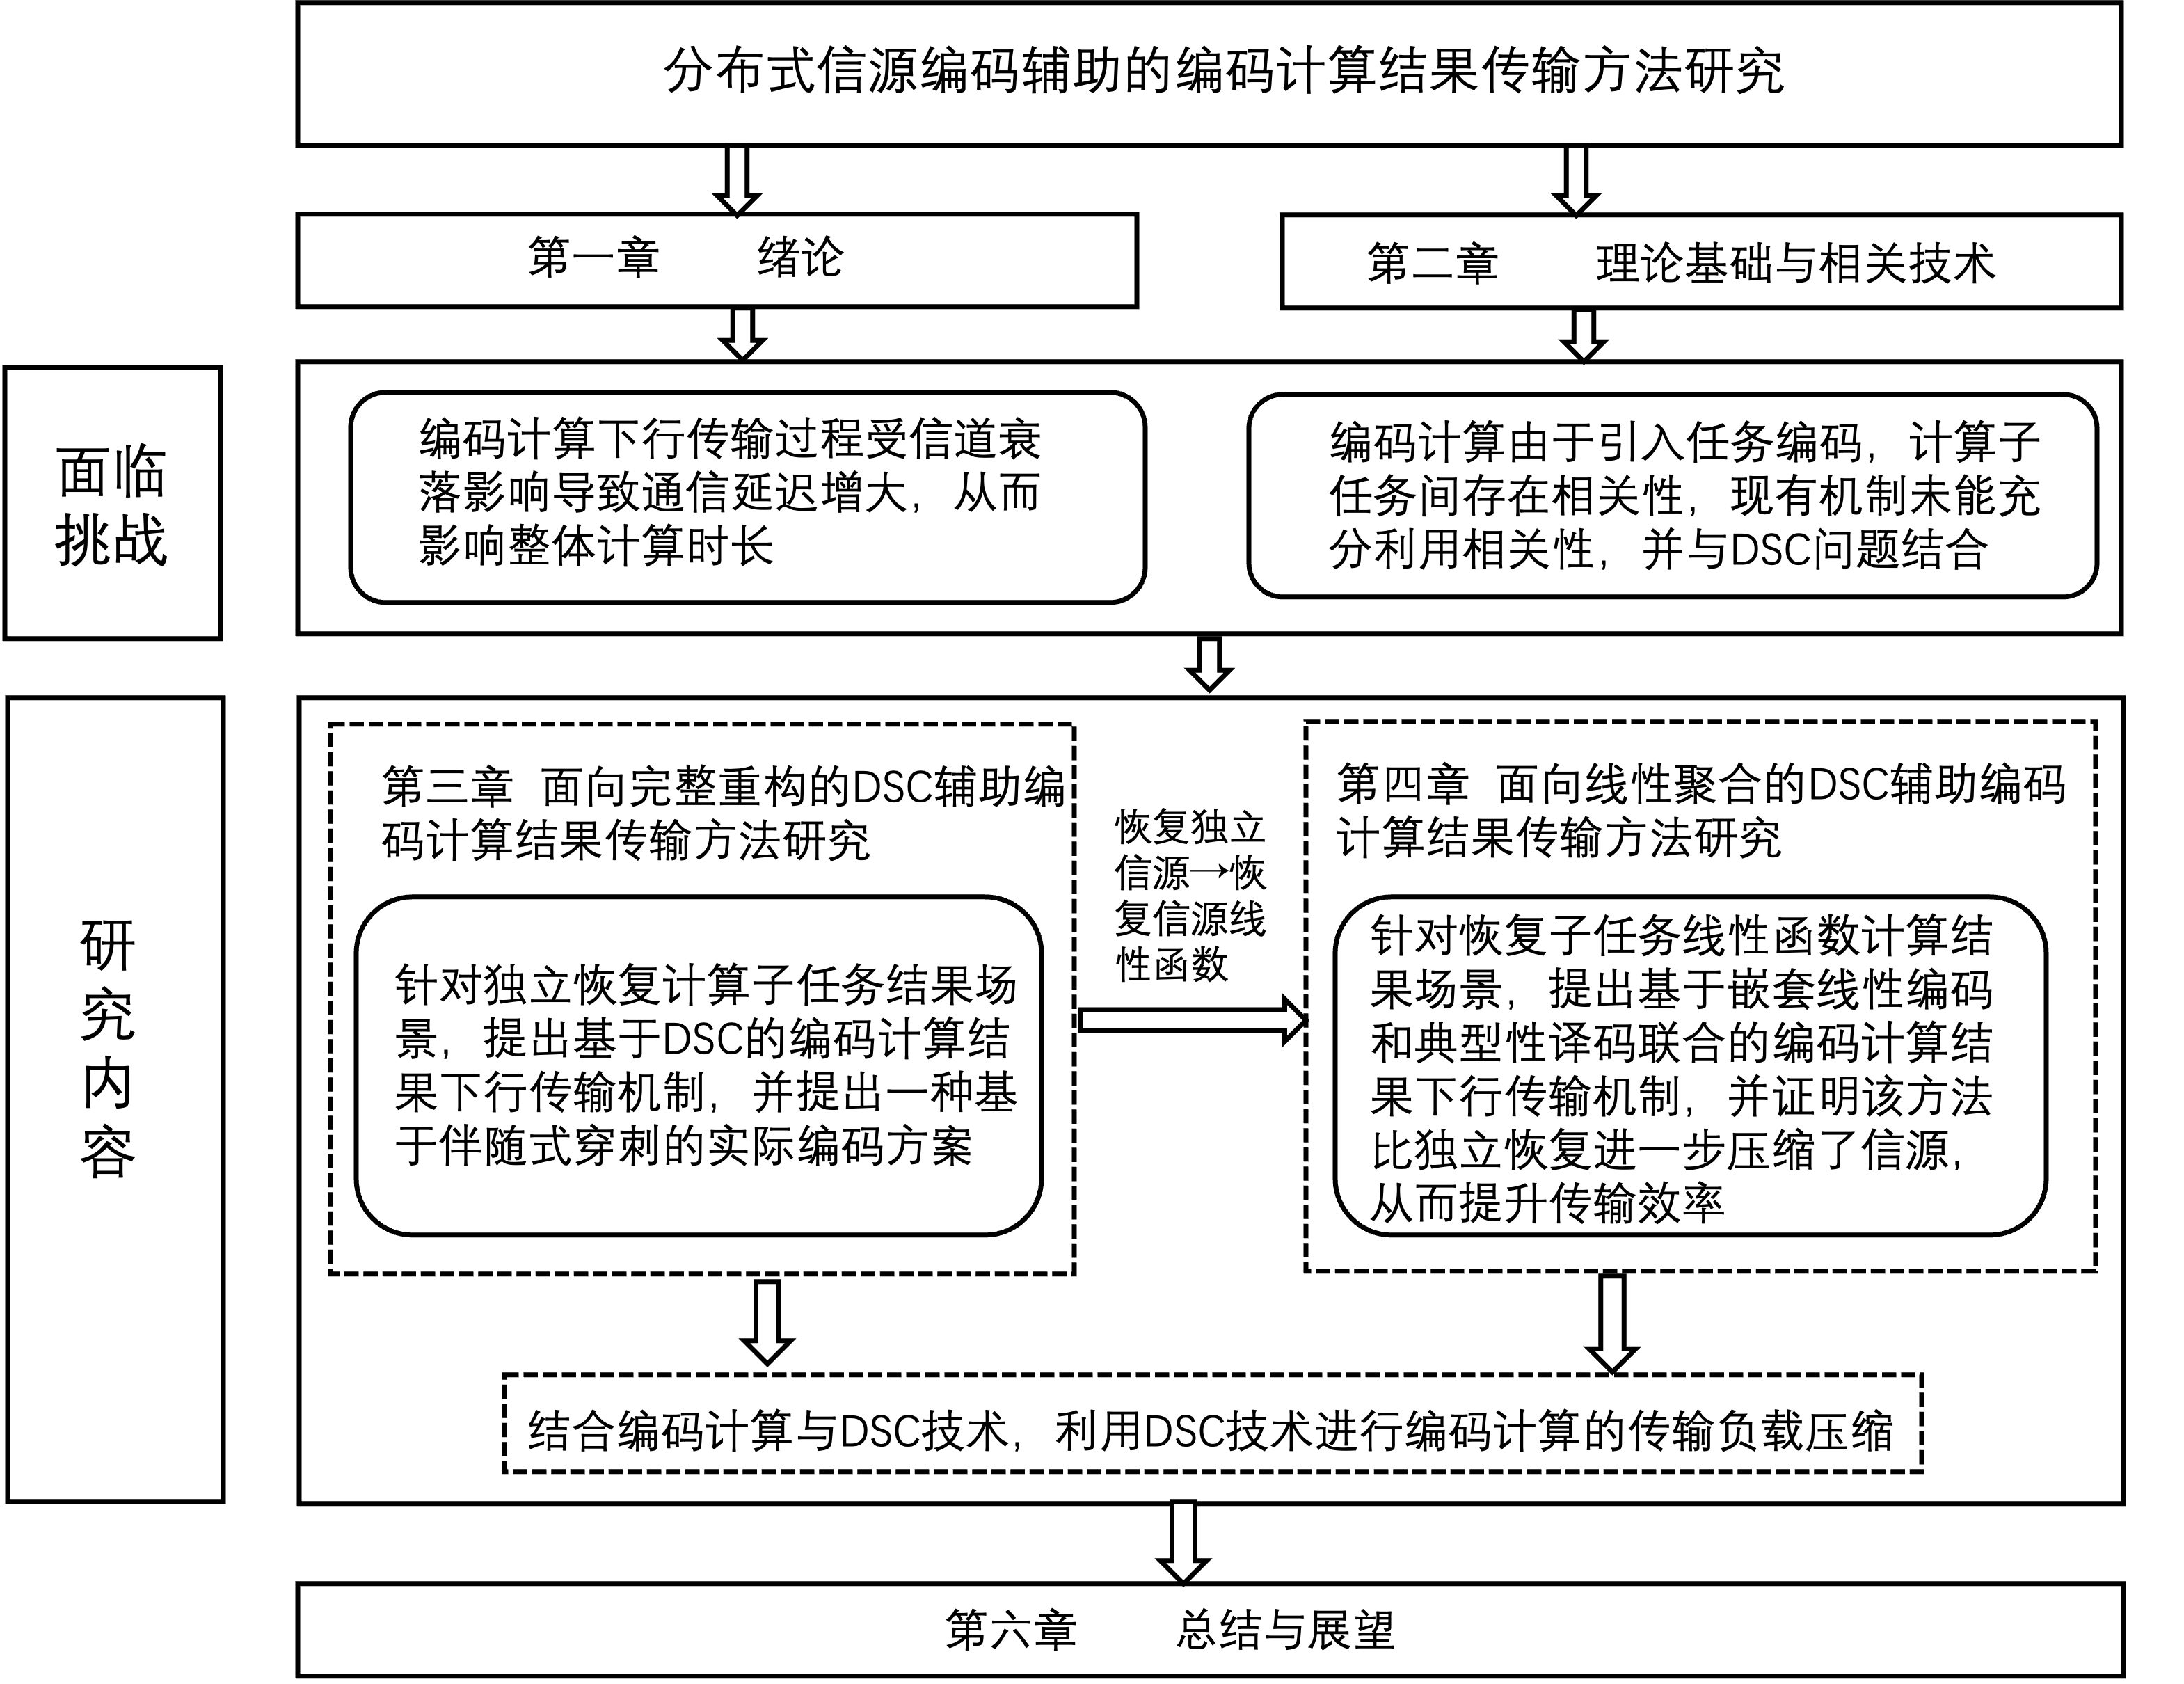
\includegraphics[width=0.97\textwidth]{研究内容与结构.png}
    \caption{本文组织结构与安排}
    \label{figure-origanization}
\end{figure}

根据上述研究内容，本文的各章节联系如\ref{figure-origanization}所示。具体内容安排如下：

第一章，绪论。该章节介绍了分布式信源编码辅助的编码计算结构方法的研究背景与意义，并总结了编码计算方法、编码计算中无线通信机制以及DSC问题的研究现状，分析了现有机制存在的问题。

第二章，理论基础与相关技术。该章节首先介绍了编码计算的基本概念以及梯度编码的编码计算方法以及无损DSC的基本概念以及针对线性函数计算的信源编码方法。随后介绍了编码计算的下行过程传输技术采用的非正交多址技术，以及最优化理论与方法，为本文后续的各研究内容问题建模和求解提供了理论基础。

第三章，面向完整重构的DSC辅助编码计算结果传输方法。针对独立恢复计算子任务结果的场景，该章节提出了基于DSC的编码计算结果下行传输机制。首先，基于理论信源压缩极限，对编码计算下行传输过程进行建模。为了实现信源压缩，之后该章节提出了基于伴随式穿刺的具体DSC方案，并推导出了该方案对应的压缩区域。随后，该章节将所提机制扩展到了高维数据的场景。基于上述机制，本章建模了相应的编码计算最小化下行传输延迟问题，利用凹凸过程对该问题进行求解，在此基础上，本章提出了问题求解的优化算法，并通过数值仿真结果验证了所提机制的有效性。

第四章，面向线性聚合的DSC辅助编码计算结果传输方法研究。针对恢复子任务线性函数计算场景，本章提出了面向线性恢复的DSC辅助编码计算结果下行传输机制。给出了基于嵌套线性码编码和典型性译码下的信源压缩极限，并基于该极限值进行了编码计算下行传输最小化优化问题的建模。随后，提出了具体的优化算法，并通过数值仿真验证所提机制的有效性。

第五章，总结与展望。该章节对本文的研究内容进行了总结，并进一步探讨了DSC应用编码计算的更多研究方向。

